\documentclass[oneside,a4paper,14pt]{extarticle}
\usepackage[T1,T2A]{fontenc}
\usepackage[
a4paper,
letterpaper,
top=2cm,
bottom=2cm,
left=2.5cm,
right=1.5cm
]{geometry}
\usepackage[utf8]{inputenc}
\usepackage[russian]{babel}
\usepackage{textcomp}
\usepackage{indentfirst}
\usepackage{listings}
\usepackage{xcolor}
\usepackage{enumitem}
\usepackage{graphicx}
\usepackage{mwe}
\usepackage{wrapfig}
\usepackage{caption}
\usepackage{amsmath}
\usepackage{amsfonts}
\usepackage{float}
\usepackage{amsthm}
\usepackage[all]{xy}
\usepackage[breaklinks]{hyperref}
\usepackage{titlesec}
\usepackage{adjustbox}
\titleformat{\section}
{\normalsize\bfseries}
{\thesection} {1em}{}
\titleformat{\subsection}
{\normalsize\bfseries}
{\thesubsection} {1em}{}
\titleformat{\subsubsection}
{\normalsize\bfseries}
{\thesubsubsection} {1em}{}
\renewcommand\baselinestretch{1.33}
\normalsize
\setlength{\parindent}{1.25cm}
\lstset{
	language=SQL,
	basicstyle=\ttfamily\small,
	keywordstyle=\color{blue},
	commentstyle=\color{green!60!black},
	stringstyle=\color{red},
	numbers=left,
	numberstyle=\tiny\color{gray},
	frame=single,
	breaklines=true,
	showstringspaces=false,
	tabsize=4,
	inputencoding=utf8,
	extendedchars=true,
	literate={а}{{\selectfont\char224}}1 {б}{{\selectfont\char225}}1 {в}{{\selectfont\char226}}1 {г}{{\selectfont\char227}}1 {д}{{\selectfont\char228}}1 {е}{{\selectfont\char229}}1 {ж}{{\selectfont\char230}}1 {з}{{\selectfont\char231}}1 {и}{{\selectfont\char232}}1 {й}{{\selectfont\char233}}1 {к}{{\selectfont\char234}}1 {л}{{\selectfont\char235}}1 {м}{{\selectfont\char236}}1 {н}{{\selectfont\char237}}1 {о}{{\selectfont\char238}}1 {п}{{\selectfont\char239}}1 {р}{{\selectfont\char240}}1 {с}{{\selectfont\char241}}1 {т}{{\selectfont\char242}}1 {у}{{\selectfont\char243}}1 {ф}{{\selectfont\char244}}1 {х}{{\selectfont\char245}}1 {ц}{{\selectfont\char246}}1 {ч}{{\selectfont\char247}}1 {ш}{{\selectfont\char248}}1 {щ}{{\selectfont\char249}}1 {ъ}{{\selectfont\char250}}1 {ы}{{\selectfont\char251}}1 {ь}{{\selectfont\char252}}1 {э}{{\selectfont\char253}}1 {ю}{{\selectfont\char254}}1 {я}{{\selectfont\char255}}1 {А}{{\selectfont\char192}}1 {Б}{{\selectfont\char193}}1 {В}{{\selectfont\char194}}1 {Г}{{\selectfont\char195}}1 {Д}{{\selectfont\char196}}1 {Е}{{\selectfont\char197}}1 {Ж}{{\selectfont\char198}}1 {З}{{\selectfont\char199}}1 {И}{{\selectfont\char200}}1 {Й}{{\selectfont\char201}}1 {К}{{\selectfont\char202}}1 {Л}{{\selectfont\char203}}1 {М}{{\selectfont\char204}}1 {Н}{{\selectfont\char205}}1 {О}{{\selectfont\char206}}1 {П}{{\selectfont\char207}}1 {Р}{{\selectfont\char208}}1 {С}{{\selectfont\char209}}1 {Т}{{\selectfont\char210}}1 {У}{{\selectfont\char211}}1 {Ф}{{\selectfont\char212}}1 {Х}{{\selectfont\char213}}1 {Ц}{{\selectfont\char214}}1 {Ч}{{\selectfont\char215}}1 {Ш}{{\selectfont\char216}}1 {Щ}{{\selectfont\char217}}1 {Ъ}{{\selectfont\char218}}1 {Ы}{{\selectfont\char219}}1 {Ь}{{\selectfont\char220}}1 {Э}{{\selectfont\char221}}1 {Ю}{{\selectfont\char222}}1 {Я}{{\selectfont\char223}}1,
}
\begin{document}
	\newpage\thispagestyle{empty}
	\begin{center}
		МИНИСТЕРСТВО НАУКИ И ВЫСШЕГО ОБРАЗОВАНИЯ\\
		РОССИЙСКОЙ ФЕДЕРАЦИИ\\
		ФЕДЕРАЛЬНОЕ ГОСУДАРСТВЕННОЕ БЮДЖЕТНОЕ\\
		ОБРАЗОВАТЕЛЬНОЕ УЧРЕЖДЕНИЕ ВЫСШЕГО ОБРАЗОВАНИЯ\\
		<<ВЯТСКИЙ ГОСУДАРСТВЕННЫЙ УНИВЕРСИТЕТ>>\\
		Институт математики и информационных систем\\
		Факультет автоматики и вычислительной техники\\
		Кафедра электронных вычислительных машин
	\end{center}
	\vspace{20mm}
	\begin{center}
		Отчёт по лабораторной работе №3\\
		по дисциплине\\
		<<Базы данных>>\\
	\end{center}
	\vspace{48mm}
	\noindent
	Выполнил студент гр. ИВТб-2303-06-00 \hfill \rule[-0,5mm]{30mm}{0.15mm}\,/Шубин В. Ю./
	\newline
	Проверил преподаватель кафедры ЭВМ \hfill \rule[-0,5mm]{30mm}{0.15mm}\,/Клюкин В. Л./
	\vfill
	\begin{center}
		Киров\\
		2026
	\end{center}
	\newpage
	\thispagestyle{empty}
	\section*{Цель работы:} Познакомиться с созданием пользовательских функций и триггеров в PostgreSQL, освоить работу с составными типами данных и массивами, изучить основы работы с процедурным языком PL/pgSQL.
	
	\section*{Среда разработки:} PostgreSQL 18, pgAdmin 4, Windows 10.
	
	\newpage
	
	\section*{Задание 1. Функция save\_game}
	
	Функция принимает параметры, соответствующие столбцам таблицы game. Если переданный id равен NULL, выполняется INSERT, иначе --- UPDATE. Возвращает id вставленной или изменённой строки.
	
	\begin{lstlisting}
		CREATE OR REPLACE FUNCTION lab_schema.save_game(
		_id BIGINT,
		_title VARCHAR(150),
		_developer_id BIGINT,
		_release_year INTEGER,
		_price NUMERIC(10, 2),
		_is_released BOOLEAN
		)
		RETURNS BIGINT AS $$
		DECLARE
		used_id BIGINT;
		BEGIN
		IF _id IS NULL THEN
		INSERT INTO lab_schema.game (title, developer_id, release_year, price, is_released)
		VALUES (_title, _developer_id, _release_year, _price, _is_released)
		RETURNING id INTO used_id;
		ELSE
		UPDATE lab_schema.game
		SET title = _title,
		developer_id = _developer_id,
		release_year = _release_year,
		price = _price,
		is_released = _is_released
		WHERE id = _id;
		used_id := _id;
		END IF;
		RETURN used_id;
		END;
		$$ LANGUAGE plpgsql;
		
		-- Тест: добавление новой игры (INSERT)
		SELECT lab_schema.save_game(NULL, 'Elden Ring', 1, 2022, 59.99, true);

	\end{lstlisting}
	
	Результат работы функции представлен на рисунке~1.
	
	\begin{figure}[H]
		\centering
		\adjustbox{max width=\linewidth}{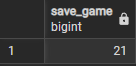
\includegraphics{s1.png}}
		\caption{Результат работы функции save\_game}
	\end{figure}
	
	\newpage
	
	\section*{Задание 2. Функция delete\_developer}
	
	Функция принимает id строки и удаляет её из таблицы developer. Если на удаляемую строку существуют внешние ссылки, функция поднимает ошибку.
	
	\begin{lstlisting}
		CREATE OR REPLACE FUNCTION lab_schema.delete_developer(
		_id BIGINT
		)
		RETURNS VOID AS $$
		BEGIN
		DELETE FROM lab_schema.developer WHERE id = _id;
		EXCEPTION
		WHEN foreign_key_violation THEN
		RAISE EXCEPTION 'Невозможно выполнить удаление, так как есть внешние ссылки.';
		END;
		$$ LANGUAGE plpgsql;
		
		-- Тест: попытка удаления разработчика с внешними ссылками
		SELECT lab_schema.delete_developer(1);
	\end{lstlisting}
	
	Результат работы функции представлен на рисунке~2.
	
	\begin{figure}[H]
		\centering
		\adjustbox{max width=\linewidth}{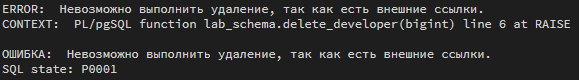
\includegraphics{s2.png}}
		\caption{Результат работы функции delete\_developer}
	\end{figure}
	
	\newpage
	
	\section*{Задание 3. Функция фильтрации по числовому значению}
	
	Функция принимает минимальное значение цены и возвращает множество строк из таблицы game, где цена больше или равна переданному значению.
	
	\begin{lstlisting}
		CREATE OR REPLACE FUNCTION lab_schema.filter_games_by_price(
		_min_price NUMERIC(10, 2)
		)
		RETURNS SETOF lab_schema.game AS $$
		BEGIN
		RETURN QUERY
		SELECT * FROM lab_schema.game
		WHERE price >= _min_price;
		END;
		$$ LANGUAGE plpgsql;
		
		-- Тест: игры с ценой >= 20
		SELECT * FROM lab_schema.filter_games_by_price(20.00);
	\end{lstlisting}
	
	Результат работы функции представлен на рисунке~3.
	
	\begin{figure}[H]
		\centering
		\adjustbox{max width=\linewidth}{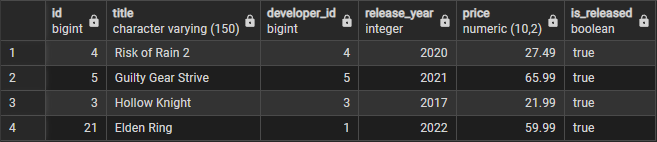
\includegraphics{s3.png}}
		\caption{Результат работы функции filter\_games\_by\_price}
	\end{figure}
	
	\newpage
	
	\section*{Задание 4. Составной тип и фильтрация массива}
	
	Создан составной тип t\_game, содержащий поля id, title и price. Функция принимает массив объектов этого типа и минимальное значение цены, возвращает отфильтрованный массив.
	
	\begin{lstlisting}
		CREATE TYPE lab_schema.t_game AS (
		id BIGINT,
		title VARCHAR(150),
		price NUMERIC(10, 2)
		);
		
		CREATE OR REPLACE FUNCTION lab_schema.filter_games_array(
		_arr lab_schema.t_game[],
		_min_price NUMERIC(10, 2)
		)
		RETURNS lab_schema.t_game[] AS $$
		BEGIN
		RETURN ARRAY(
		SELECT (id, title, price)::lab_schema.t_game
		FROM unnest(_arr)
		WHERE price >= _min_price
		);
		END;
		$$ LANGUAGE plpgsql;
		
		-- Тест: фильтрация массива всех игр по цене >= 30
		SELECT lab_schema.filter_games_array(
		ARRAY(
		SELECT (id, title, price)::lab_schema.t_game
		FROM lab_schema.game
		),
		30.00
		);
	\end{lstlisting}
	
	Результат работы функции представлен на рисунке~4.
	
	\begin{figure}[H]
		\centering
		\adjustbox{max width=\linewidth}{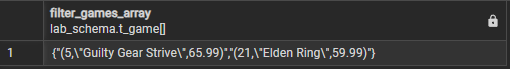
\includegraphics{s4.png}}
		\caption{Результат работы функции filter\_games\_array}
	\end{figure}
	
	\newpage
	
	\section*{Задание 5. Таблица log\_game и триггеры}
	
	Создана таблица log\_game для логирования изменений цены в таблице game. Реализованы триггерная функция и триггер, срабатывающий после INSERT или UPDATE.
	
	\begin{lstlisting}
		CREATE TABLE lab_schema.log_game (
		id BIGSERIAL PRIMARY KEY,
		game_id BIGINT REFERENCES lab_schema.game(id),
		change_datetime TIMESTAMP DEFAULT NOW(),
		old_price NUMERIC(10, 2) DEFAULT NULL,
		new_price NUMERIC(10, 2) DEFAULT NULL
		);
		
		CREATE OR REPLACE FUNCTION lab_schema.log_game_price_trigger()
		RETURNS TRIGGER AS $$
		DECLARE
		old_val NUMERIC(10, 2);
		BEGIN
		IF (TG_OP = 'UPDATE') THEN
		old_val := OLD.price;
		ELSIF (TG_OP = 'INSERT') THEN
		old_val := NULL;
		END IF;
		
		INSERT INTO lab_schema.log_game (game_id, old_price, new_price)
		VALUES (NEW.id, old_val, NEW.price);
		
		RETURN NEW;
		END;
		$$ LANGUAGE plpgsql;
		
		CREATE TRIGGER game_price_change_trigger
		AFTER UPDATE OR INSERT ON lab_schema.game
		FOR EACH ROW
		EXECUTE PROCEDURE lab_schema.log_game_price_trigger();
		
		-- Тест: вставка новой игры
		INSERT INTO lab_schema.game (title, developer_id, release_year, price, is_released)
		VALUES ('Test Game', 1, 2025, 19.99, true);
		
		-- Тест: изменение цены
		UPDATE lab_schema.game SET price = 24.99 WHERE title = 'Test Game';
		
		-- Проверка лога
		SELECT * FROM lab_schema.log_game;
	\end{lstlisting}
	
	Результат работы триггера представлен на рисунке~5.
	
	\begin{figure}[H]
		\centering
		\adjustbox{max width=\linewidth}{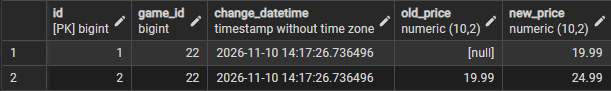
\includegraphics{s5.png}}
		\caption{Содержимое таблицы log\_game после изменений}
	\end{figure}
	
	\newpage
	
	\section*{Задание 6. Динамический запрос}
	
	Функция принимает название таблицы, название столбца и id, возвращает текстовое значение указанного поля.
	
	\begin{lstlisting}
		CREATE OR REPLACE FUNCTION lab_schema.get_value_by_id(
		_table_name VARCHAR,
		_column_name VARCHAR,
		_id BIGINT
		)
		RETURNS TEXT AS $$
		DECLARE
		result TEXT;
		BEGIN
		EXECUTE 'SELECT ' || _column_name || ' FROM lab_schema.' || _table_name || ' WHERE id = $1'
		USING _id
		INTO result;
		RETURN result;
		END;
		$$ LANGUAGE plpgsql;

		
		-- Тест: получить страну разработчика с id = 1
		SELECT lab_schema.get_value_by_id('developer', 'country', 1);
	\end{lstlisting}
	
	Результат работы функции представлен на рисунке~6.
	
	\begin{figure}[H]
		\centering
		\adjustbox{max width=\linewidth}{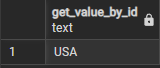
\includegraphics{s6.png}}
		\caption{Результат работы функции get\_value\_by\_id}
	\end{figure}
	
	\newpage
	
	\section*{Выводы} В ходе выполнения лабораторной работы были освоены создание пользовательских функций и триггеров в PostgreSQL. Реализована функция save\_game для вставки и обновления записей с использованием конструкции RETURNING. Создана функция delete\_developer с обработкой исключений для проверки ссылочной целостности. Освоена работа с составными типами данных и массивами: создан тип t\_game и функция фильтрации массива объектов. Реализована таблица log\_game и триггеры для логирования изменений числового поля. Изучены динамически формируемые запросы с использованием EXECUTE и конструкции USING. Все функции реализованы на процедурном языке PL/pgSQL и успешно протестированы.
	
\end{document}